\chapter{基于输入扰动的神经网络不确定性研究}


\section{引言}
对神经网络不确定性的研究,可以在模型无法准确预测时给出一个不确定性值,辅助决策,对于高不确定性的预测,引入人力监控,降低风险。目前对神经网络的不确定性建模方法中,以模型集成类方法表现最好,但是模型集成类方法需要训练和保存多个模型,存储和计算成本较高,为了更高效地计算神经网络的不确定性,使用单一确定性的神经网络通过一次预测建模不确定性逐渐成为神经网络不确定性研究的热点。在单一确定性神经网络建模不确定性的方法中,一种思路是通过概率密度建模的方法计算模型的不确定性,这类方法的基本思想是分布内的样本应该具有高的概率密度值,而对于分布外样本由于提取的特征偏离所构建的多维概率分布,所以具有较低的概率密度,因此在多维概率分布上的概率密度可以作为模型不确定性的度量。在这类方法中DDU\cite{Mukhoti_2023_CVPR}算法是最新的研究成果,DDU算法通过在训练模型时对网络的权重使用谱归一化操作,得到归一化的高维特征空间,并在训练集的高维特征空间上使用高斯混合模型(Gaussian Mixture Model,GMM)构建一个经验的多维概率分布,当一个新的样本输入训练好的神经网络提取得到高维特征,该高维特征在所构建的经验概率分布上所计算的概率密度可以作为模型不确定性的度量。但是DDU算法仍然存在着缺点,其一作者指出该算法在含有残差结构的神经网络上表现较好,对于其他的网络(如VGG)建模的不确定性的效果较差,其二在多个数据集上测试结果表明DDU算法相距模型集成类算法在建模网络不确定性上仍有一定差距。


本文的主要思路同样是基于高维特征的概率密度建模神经网络的模型不确定性,使用在训练集上神经网络提取的高维特征,构建一个多维概率分布,测试样本经过神经网络得到一个高维特征,通过计算测试样本高维特征经验概率分布上的概率密度建模神经网络的模型不确定性。为了改进DDU算法对模型不确定性的建模效果,并提高在代理评估任务上的表现,本章首先从梯度空间入手,研究训练集样本和分布外样本在梯度空间上的分布差异,通过可视化输出关于输入的梯度响应图,观察到对于分布外样本,梯度响应明显的大于分布内样本,从这一结论出发,即基于剃度空间上分布内样本和分布外样本的梯度响应差异性,提出基于输入扰动的改进,通过对输入图片加入与梯度响应相关的输入扰动,然后重新计算概率密度,作为模型不确定性的度量。由于对于分布内样本,输入扰动很微小,但是对于分布外样本,输入扰动很明显,所以可以拉开分布内样本和分布外样本在多维概率分布上的差异。具体的算法框架见\ref{tag:模型结构图1}。

为了评估本文提出的基于输入扰动的改进,本章后续分别在OOD检测,误分类样本识别,对抗样本检测,主动学习等代理任务上实验,在这些任务上的实验结果验证了基于输入扰动的改进对基于高维特征概率密度建模不确定性所带来的提升。


\begin{figure}[h]
    \centering
    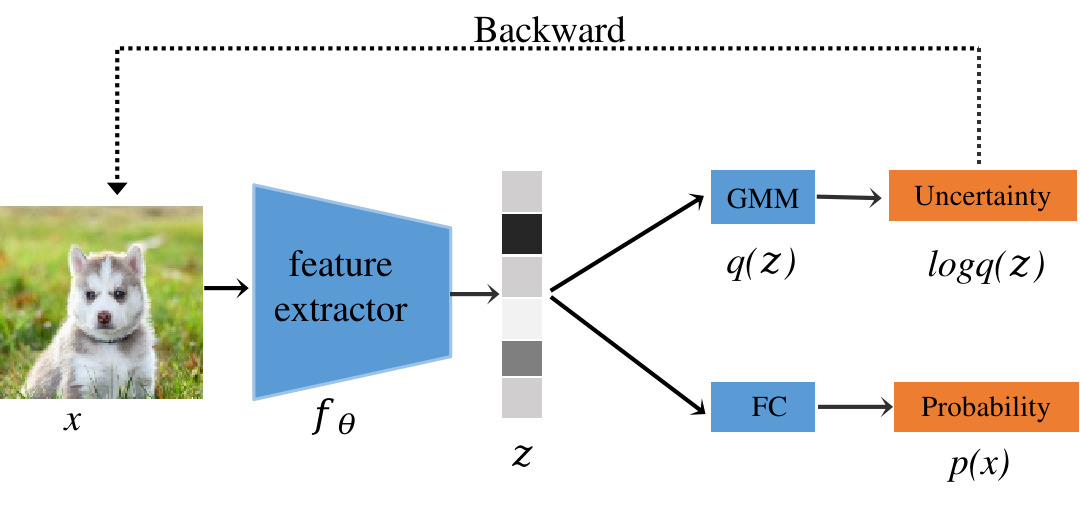
\includegraphics[width=1.\linewidth]{assets/structure1.png}
    \caption{基于高维特征概率密度建模的模型不确定性}
    \label{tag:模型结构图1}
\end{figure}

% \begin{figure}[h]
%     \centering
%     \begin{tikzpicture}[
%         node distance=1.5cm and 1.5cm,
%         every node/.style={minimum height=1.2cm, text width=2.0cm, align=center},
%         feature/.style={fill=blue!20},
%         gmm/.style={fill=orange!50,text width={1.0cm}},
%         fc/.style={fill=orange!50,text width={1.0cm}},
%         softmax/.style={fill=orange!50},
%         output/.style={fill=gray!30},
%         arrow/.style={-{Stealth[scale=1.2]}},
%         backward/.style={dashed, red, thick} % 红色虚线样式
%     ]
%     % Nodes
%     \node (image) {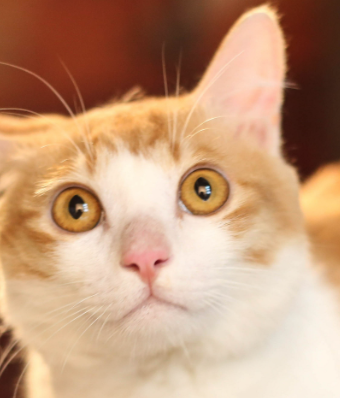
\includegraphics[width=1.5cm]{assets/cat.png}};
%     \node[below=0.2cm of image, align=center] (input_label) {输入$x$};
%     \node[feature, right=of image, trapezium, trapezium angle=60, fill=blue!20, minimum width=1.8cm, minimum height=1.5cm, shape border rotate=270] (feature_extractor) {feature extractor};
%     \node[below=0.2cm of feature_extractor, align=center] (input_label) {$f_\theta$};
    
%     % 条形图节点
%     \node[right=1cm of feature_extractor, inner sep=0] (bar_chart) {
%         \begin{tikzpicture}[scale=0.9]
%             % 绘制主条
%             \draw[thick] (0,0) rectangle (0.5,5); % 外框
%             % 分块填充
%             \fill[black!80] (0,4.5) rectangle (0.5,5);
%             \fill[gray!10] (0,4.0) rectangle (0.5,4.5);
%             \fill[gray!50] (0,3.5) rectangle (0.5,4);
%             \fill[black!70] (0,3) rectangle (0.5,3.5);
%             \fill[gray!70] (0,2.5) rectangle (0.5,3);
%             \fill[gray!20] (0,2) rectangle (0.5,2.5);
%             \fill[black!40] (0,1.5) rectangle (0.5,2);
%             \fill[gray!30] (0,1) rectangle (0.5,1.5);
%             \fill[black!80] (0,0.5) rectangle (0.5,1);
%             \fill[gray!60] (0,0) rectangle (0.5,0.5);
%         \end{tikzpicture}
%     };
%     \node[below=0.2cm of bar_chart, align=center] (input_label) {$z$};

%     % 其他节点
%     \node[gmm, above right=0.001cm and 0.5cm of bar_chart] (gmm) {GMM};
%     \node[below=0.1cm of gmm, align=center] (input_label) {$q(z)$};
%     \node[fc, below right=0.001cm and 0.5cm of bar_chart] (fc) {FC};
%     % \node[softmax, right=1.0cm of fc] (softmax) {Softmax};
%     \node[output, right=1.0cm of fc] (probs) {Probs};
%     \node[below=0.1cm of probs, align=center] (input_label) {$p(x)$};
%     \node[output, right=1.0cm of gmm] (logPx) {Uncertainty};
%     \node[below=0.1cm of logPx, align=center] (input_label) {$\log q(z)$};
    
%     % Paths
%     \draw[arrow] (image) -- (feature_extractor);
%     \draw[arrow] (feature_extractor) -- (bar_chart);
%     \draw[arrow] (bar_chart) -- (gmm);
%     \draw[arrow] (bar_chart) -- (fc);
%     \draw[arrow] (gmm) -- (logPx);
%     % \draw[arrow] (fc) -- (softmax);  
%     \draw[arrow] (fc) -- (probs);

%     % Backward path
%     \draw[backward] (logPx) -- ++(90:1.5cm) coordinate (midpoint); % 红色虚线
%     \draw[backward, ->] (midpoint) -- ++(180:10cm) node[pos=0.5, above] {Backward} -| (image); % 红色虚线

%     \end{tikzpicture}
%     \caption{基于高维特征概率密度建模的模型不确定性}
%     \label{tag:模型结构图}
% \end{figure}


\section{主要方法}
\subsection{不同样本梯度响应差异性研究}
Hendrycks等人\cite{hendrycks2017a}观察到训练好的网络倾向于给InD样本一个相对更高的Softmax分数,进而提出一种无需重新训练网络的基线方法MSP,该方法使用Softmax分数表示不确定性,用于OOD样本检测。Shiyu Liang等人\cite{liang2017enhancing}在此基础上发现,在Softmax函数中使用温度缩放(temperature scaling),并且给输入加入微小的梯度相关的扰动,那么ID和OoD的Softmax分数分布就会增大差异,进而显著提高OOD样本检测性能。Wang\cite{wang2023gradient}、Rui Huang\cite{huang2021importance}、Lee\cite{lee2020gradients}也各自在研究中指出梯度信息在不确定性的度量中的作用。本章在上述研究的启发下进一步研究分布内样本和分布外样本在梯度空间上分布的规律,实验结合理论推导分析相关结论,最后通过添加一些与梯度相关的输入扰动,提高概率密度在建模神经网络模型不确定性上的效果。

本章有关神经网络的梯度空间的研究,是指神经网络反向传播时输出对输入求梯度,这里的输入,是指输入的图片。如图\ref{tag:模型结构图1},使用概率密度建模不确定性,训练好的神经网络有两个输出,一个是预测类别的概率$p(x)$,一个是计算模型不确定性的概率密度$\log q(z)$。本章分别研究了这两个输出关于输入的梯度,并通过梯度响应图的可视化分析$p(x)$和$\log q(z)$对梯度响应的区别。

首先,在梯度空间上对训练集样本和域外样本进行了统计分析,统计输出关于输入的梯度响应图。\ref{fig:resp1}是在CIFAR10上训练的ResNet50可视化后的结果,选取SVHN和LSUN作为训练集以外的样本,计算出概率密度关于输入图片的梯度,得到的梯度张量在特征维度上求均值后的结果作为梯度响应图。可以看出对于训练集上的样本,梯度响应普遍在比较小的范围,而对于训练集以外的样本(理论上来说这些样本的预测不确定性更高),梯度响应会更大,这个现象表明在关于输入的梯度空间上存在着能表征不确定性的信息。
\begin{figure}[h]
    \captionsetup{font=small, justification=centering}
    \centering
    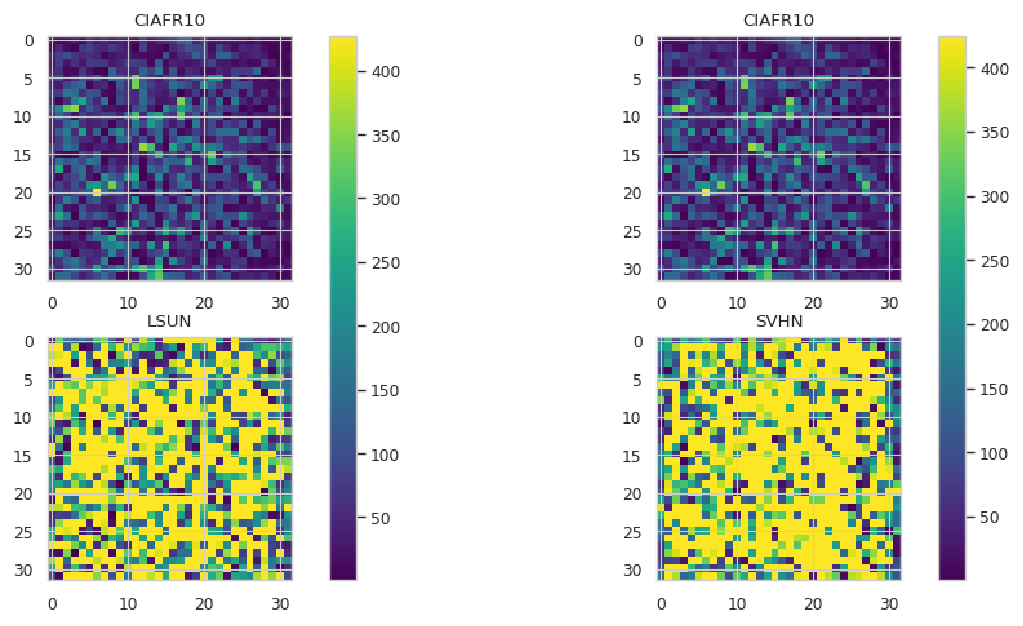
\includegraphics[width=0.75\linewidth]{assets/3-1.png}
    \caption{ResNet50 ,训练集 CIFAR10 vs OOD数据集LSUN、SVHN,概率密度关于输入的梯度响应图
}
    \label{fig:resp1}
\end{figure}

\ref{fig:resp2}是在CIFAR10上训练的VIT网络可视化梯度响应的结果,同样也是选取SVHN和LSUN作为训练集以外的样本,计算出概率密度关于输入的梯度作为梯度响应图。同样可以看出,对于基于Transformer\cite{vaswani2017attention}结构的神经网络,也有和卷积网络相同的结论,即对于训练集上的样本,关于输入的梯度响应在比较小的范围,而对于训练集以外的样本,关于输入的梯度响应会在一个更大的范围内。所以可以得出结论,对于基于Transformer结构的神经网络,关于输入的梯度空间上的信息也和模型不确定性具有相关性。
\begin{figure}[h]
    \captionsetup{font=small, justification=centering}
    \centering
    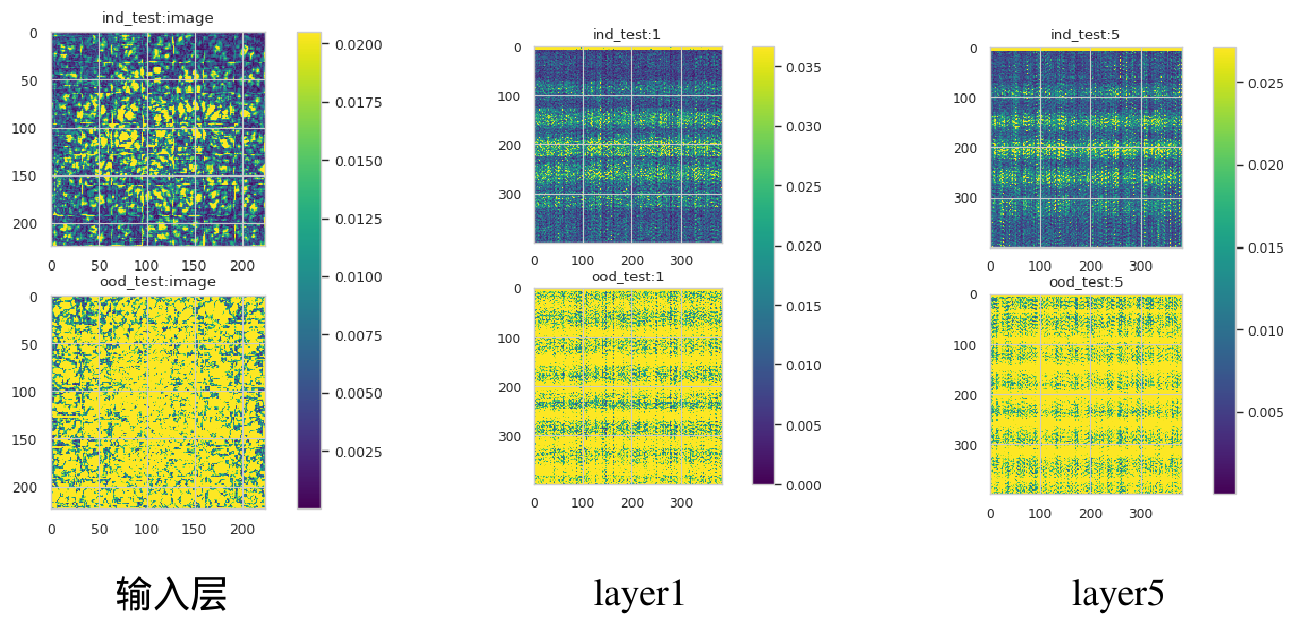
\includegraphics[width=0.75\linewidth]{assets/3-2.png}
    \caption{VIT,训练集 CIFAR10 vs OOD数据集LSUN、SVHN,概率密度关于输入的梯度响应图
}
    \label{fig:resp2}
\end{figure}

以上研究了对不同网络结构使用概率密度求关于输入的图片梯度响应的结果,如上文所言,还可以计算经过Softmax输出的预测概率对输入图片求梯度,本章同样也可视化了Softmax计算出的预测概率对输入图片的梯度。\ref{fig:resp3}是在CIFAR10上训练的ResNet50网络可视化梯度响应的结果,同样也是选取SVHN和LSUN作为训练集以外的样本,在这个实验中计算预测概率关于输入的梯度作为梯度响应图。可以看出,对于训练集上的样本,梯度响应比较小,而对于训练集以外的样本,梯度响应会在一个更大的范围内。对比图\ref{fig:resp1},同时可以发现,使用概率密度计算出来的梯度空间上的响应图,训练集和域外样本的分布差异更大,这表明使用概率密度计算出的梯度在表征不确定性上相比使用预测概率计算出来的梯度效果更好。
\begin{figure}[h]
    \captionsetup{font=small, justification=centering}
    \centering
    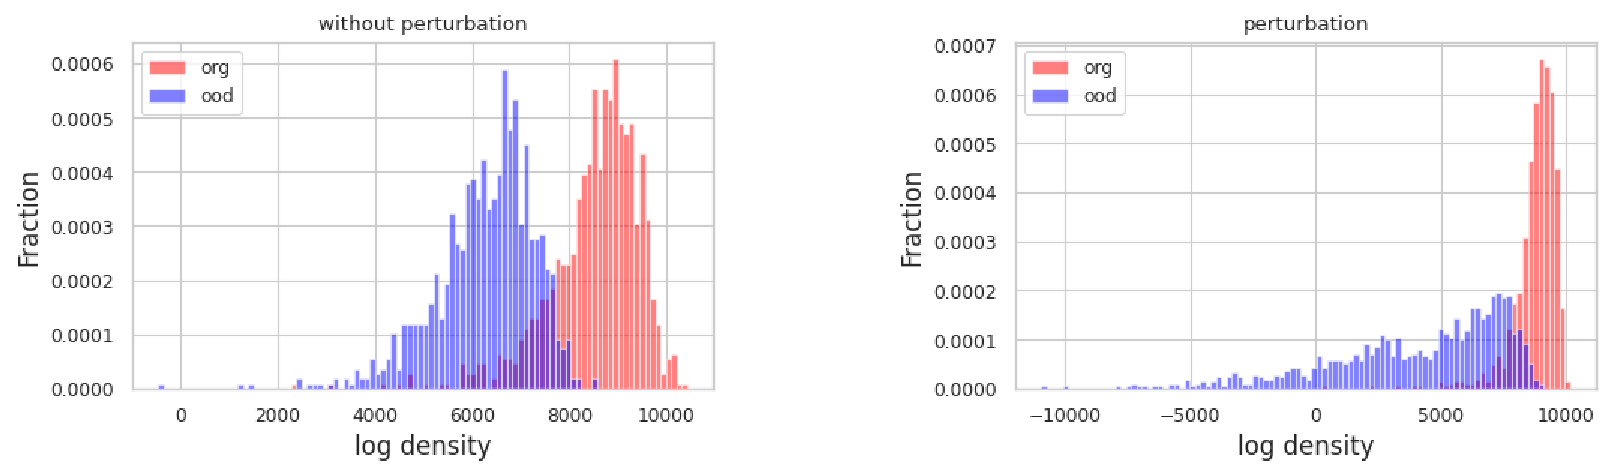
\includegraphics[width=0.75\linewidth]{assets/3-3.png}
    \caption{ResNet50,训练集 CIFAR10 vs OOD数据集LSUN、SVHN,预测概率关于输入的梯度响应图
}
    \label{fig:resp3}
\end{figure}


上面通过实验定性地观察到了对于分布内样本和分布外样本,梯度空间上存在着明显的分布差异。为了定量地分析梯度空间上的信息在建模神经网络模型不确定性上效果,本文使用计算出来的梯度张量的范数作为模型不确定性的度量,并评估在OOD检测任务上的表现。
下面是在CIFAR10数据集上训练ResNet50和VIT模型,直接使用概率密度关于输入的梯度的范数作为模型不确定性的度量,选取SVHN/LSUN/CIFAR100/MNIST作为分布外样本,在OOD检测任务上进行评估,,对比了两种方法DDU和GradNorm在OOD检测任务上的表现,通过AUROC和AUPRC两个指标评估它们在OOD检测任务上的效果,并以此间接地反映对模型不确定性的建模能力。实验结果如表\ref{tag:gradNorm}。
\begin{table}[h]
    \captionsetup{font=small, justification=centering}
    \centering
    \renewcommand{\arraystretch}{1.0} % Adjust line spacing
    \resizebox{\linewidth}{!}{
    \begin{tabular}{l l c c c}
    \toprule
    Method & OOD Dataset & VGG16+CIFAR10 & ResNet50+CIFAR10 & VIT+CIFAR10 \\
    &  & (Accuracy=0.9390) & (Accuracy=0.9558) & (Accuracy=0.9732) \\
    \midrule
    \multirow{4}{*}{DDU} 
    & SVHN & \textbf{0.9320} / \textbf{0.9480} & 0.9179 / 0.9415 &\textbf{ 0.9779} / \textbf{0.9843} \\
    & LSUN & \textbf{0.9160 }/ 0.9274 & \textbf{0.9239} /\textbf{ 0.9390} & \textbf{0.9906} /\textbf{ 0.9917} \\
    & CIFAR100 &\textbf{ 0.8932} / \textbf{0.9030} & \textbf{0.8888 }/\textbf{ 0.9018} & \textbf{0.9567} / \textbf{0.9605} \\
    & MNIST &\textbf{ 0.9195 }/ \textbf{0.9225 }& \textbf{0.9292 }/\textbf{ 0.9511 }& \textbf{0.9823 }/ \textbf{0.9854} \\
    \midrule
    \multirow{4}{*}{GradNorm} 
    & SVHN & 0.9308 / 0.9466 & \textbf{0.9282} / \textbf{0.9506} &  0.9325 / 0.9493 \\
    & LSUN & 0.9155 / \textbf{0.9326} & 0.9079/ 0.9300 & 0.8187 /  0.8755 \\
    & CIFAR100 & 0.8898 / 0.8987 & 0.8790 / 0.8955 & 0.9463/ 0.9495 \\
    & MNIST & 0.9010 / 0.9082 & 0.8958/ 0.9248 & 0.6787 / 0.7923 \\
    \bottomrule
    \end{tabular}
    }
    \caption{在CIFAR10上训练不同的模型(VGG16,ResNet50,VIT),选取SVHN、LSUN、CIFAR100、MNIST作为OOD样本,对比DDU和梯度范数(GradNorm)对模型不确定性的建模效果,报告指标是AUROC($\uparrow$) / AUPRC($\uparrow$)}
    \label{tag:gradNorm}
\end{table}


从实验结果来看,无论是对于卷积网络结构的ResNet50模型,还是基于Transformer结构的VIT模型,都可以观察到,概率密度关于输入的梯度的范数可以作为OOD检测指标并具有良好的表现,这说明概率密度关于输入的梯度对模型的不确定性具有一定的建模能力,但是对比DDU方法对OOD检测任务上的表现可以看到,DDU方法在几乎所有数据集上均表现优异,AUROC/AUPRC值均高于梯度范数在OOD检测任务上的表现,这说明直接使用梯度范数作为不确定性的度量效果不如DDU算法。

针对上面观察到的分布内样本和分布外样本在梯度空间上的分布差异,下面从理论上进行推导分析。首先,关于概率密度关于输入的梯度有以下结论:

\textbf{性质1:}
已知 \( z = f_\theta(x) \), \( q(z) = N(z|\mu_c, \Sigma_c) \),以及 \( U(x) = \log q(z) \)。 \( U(x) \) 对 \( x \) 的梯度 \( \nabla_x U(x) \):\[
\nabla_x U(x) = - \frac{\partial z}{\partial x}^T \Sigma_c^{-1} \left( z - \mu_c \right)
\]

\textbf{证明1:}根据 \( q(z) \) 的定义为正态分布的概率密度函数可知:
\[
q(z) = N(z|\mu_c, \Sigma_c) = \frac{1}{(2\pi)^{D/2}|\Sigma_c|^{1/2}} \exp\left(-\frac{1}{2}(z - \mu_c)^T \Sigma_c^{-1} (z - \mu_c) \right)
\]


\( U(x) = \log q(z) \) 的取对数展开后:
\[
U(x) = \log q(z) = -\frac{D}{2} \log(2\pi) - \frac{1}{2} \log |\Sigma_c| - \frac{1}{2}(z - \mu_c)^T \Sigma_c^{-1} (z - \mu_c)
\]


令 \( z = f_\theta(x) \),则 \( \nabla_x z = \frac{\partial z}{\partial x} = J \),其中 \( J \) 是 \( z \) 对 \( x \) 的雅可比矩阵。

\( U(x) \) 中与 \( x \) 相关的部分为:
\[
-\frac{1}{2}(z - \mu_c)^T \Sigma_c^{-1} (z - \mu_c)
\]

对 \( x \) 求梯度:
\[
\nabla_x U(x) = -\frac{1}{2} \nabla_x \left[ (z - \mu_c)^T \Sigma_c^{-1} (z - \mu_c) \right]
\]

对括号内的二次型展开:
\[
(z - \mu_c)^T \Sigma_c^{-1} (z - \mu_c) = \text{tr} \left[ \Sigma_c^{-1} (z - \mu_c) (z - \mu_c)^T \right]
\]

利用链式法则:
\[
\nabla_x \left[ (z - \mu_c)^T \Sigma_c^{-1} (z - \mu_c) \right] = 2 J^T \Sigma_c^{-1} (z - \mu_c)
\]

因此:
\[
\nabla_x U(x) = -J^T \Sigma_c^{-1} (z - \mu_c)
\]

最终结果可以写为:
\[
\nabla_x U(x) = - \frac{\partial z}{\partial x}^T \Sigma_c^{-1} \left( z - \mu_c \right)
\]

其中:\( z = f_\theta(x) \),\( J = \frac{\partial z}{\partial x} \) 是雅可比矩阵,\( \Sigma_c^{-1} \) 是协方差矩阵的逆,\( \mu_c \) 是均值向量。

分析上述推导结果,第一项主要是神经网络参数有关,由于对不同的输入统一使用训练好的确定网络,参数也是确定的,所以在分析分布内样本和分布外样本的梯度响应时,重要的因素是 \( (z - \mu_c) \) 和 \( \Sigma_c^{-1} \) 的相互作用。 对于分布内样本,其 \( z \) 接近于类别的均值 \( \mu_c \)。由于 \( z \) 离均值较近,\( (z - \mu_c) \) 的值较小,从而导致梯度较小,即梯度响应会相对较弱。这是因为分布内的样本已经在类别的集中区域,因此梯度计算时主要影响的是样本到均值的微小偏差。对于分布外样本,其 \( z \) 会远离类别的均值 \( \mu_c \),导致 \( (z - \mu_c) \) 的值较大。此时,梯度的响应较强,因为样本 \( z \) 相对于均值的距离较大。换句话说,分布外样本的梯度变化率较高,因为它们距离类别中心较远,模型对于这些样本的变化响应更为显著。


\subsection{基于输入扰动的改进}
基于上一节关于不同分布的样本在梯度空间上的实验观察和理论分析,可以知道域内样本和域外样本在梯度空间上的分布存在着明显差异,在域内测试样本上概率密度对输入图片的梯度响应处在一个很低的范围内,而域外测试样本概率密度对输入图片的梯度响应处在一个很高的范围。基于梯度空间上域内样本和域外样本存在的分布差异,本节对DDU算法建模不确定性提出基于输入扰动的改进,基本思想是由于域内样本梯度响应比较小而域外样本梯度响应比较大,同时对输入图片加入与梯度相关的输入扰动,对域外样本的影响更大,偏离在训练集上所构建的经验分布,进而导致域内样本和域外样本在所构建分布上的分布差异将会变大。

基于高维特征的概率密度建模神经网络的模型不确定性,通过高斯混合模型(GMM)建模高维特征空间的概率分布$q(z)$,

\begin{equation}
N(z|\mu_c,\Sigma_c)=\frac{1}{(2\pi)^{D/2}}\frac{1}{\left| \Sigma_c \right|^{1/2}}exp\left\{-\frac{1}{2}(z-\mu_c)^T\Sigma_c^{-1}(z-\mu_c)\right\}
\end{equation}
\begin{equation}
    q(z)  = \sum_{c=1}^{K}w_cN(z|\mu_c,\Sigma_c)
\end{equation}
并利用测试样本在所建概率分布上的概率密度来评估模型的不确定性。

具体而言,在\textbf{训练阶段},需要首先训练一个高准确率的神经网络,使用训练好的骨干网络对训练集上的图片提取高维特征以生成训练样本的特征表示,然后为每个类别计算其高维特征的均值$\mu_c$、协方差矩阵$\Sigma_c$以及类别先验概率$q(y|c)$,从而建立一个描述特征空间分布的高斯混合模型$q(z)$。

在\textbf{不确定性计算阶段},通过特征提取网络计算测试样本$x$的高维特征表示$z$,并利用高斯混合模型估计该高维特征$z$的概率密度$\log q(z)$。 随后,对输入样本施加梯度有关的输入扰动(
添加输入扰动的方式见公式\ref{perturb})得到扰动后的输入$\tilde{x}$,使其沿着概率密度减小的方向变化,并再次计算扰动后样本的概率密度$q(\tilde{z})$,扰动后的概率密度,最终作为模型在该输入样本上的模型不确定性:$Uncertainty = logq(\tilde{z})$。

\begin{equation}
    \tilde{x}=x-\epsilon* \cdot sign(\nabla_x U(x))
    \label{perturb}
\end{equation}
其中:
\begin{equation}
    U(x)=\log q(f_{\theta}(x))
\end{equation}
超参数$\epsilon$通过网格搜索(Grid Search)优化得到。


完整的基于输入扰动的改进算法原理见\ref{alg:1}。


\begin{algorithm}[h]
	\caption{基于输入扰动的概率密度建模的模型不确定性算法}
	\label{alg:1}
	
	\begin{algorithmic}[1]
		\Require 训练集: $(X,Y)$ 
		\Require 谱归一化的高维特征提取网络: $f_{\theta}:x \rightarrow \mathbf{R}^d $ 
		\Require GMM模型: $q(z) = \max_{c}q(z|y=c)$
		
		\\
		\Procedure {1.训练阶段和GMM建模}{}
		\State 在训练数据集数据集上训练网络$f_{\theta}$
		\For {属于类别c的样本}
		\State $\mu_{c}=\frac{1}{|x_c|}f_{\theta}(x_c)$
		\State $\Sigma_c = \frac{1}{|x_c|-1}(f_{\theta}(x_c)-\mu_c)(f_{\theta}(x_c)-\mu_c)^T$
		\State q(y=c)=$\frac{|X_C|}{|X|}$
		\EndFor
		\EndProcedure

		
		\\
		\Procedure {2.模型不确定性计算}{}
		\State $z=f_{\theta}(x)$
		\State  $q(z) = \max_{c}q(z|y=c)$,其中$q(z)\sim N(\mu_c,\Sigma_c)$
		\State $\tilde{x}=x-\epsilon* \cdot sign(\nabla_x \log q(z)))$,其中$\epsilon$通过grid search调参
		\State $\tilde{z}=f_{\theta}(\tilde{x})$
		\State 计算模型不确定性 $Uncertainty(x) = \log \max_{c}q(\tilde{z}|y=c)$,其中$q(\tilde{z})\sim N(\mu_c,\Sigma_c)$
		\EndProcedure 
	\end{algorithmic}
\end{algorithm}


在实验中,对输入图像进行了梯度扰动,并重新计算了概率密度作为模型不确定性的度量。实验结果如图\ref{tag:uncertainty 1}所示,展示了输入加入扰动前后,inD样本和OOD样本模型不确定性的分布。该实验在CIFAR10数据集上训练了ResNet50模型,并在数据集上建立了高维特征的经验混合高斯分布GMM。选取CIFAR10数据集的测试集作为分布内样本(inD),SVHN、CIFAR100、MNIST、LSUN数据集的测试集作为分布外样本(OOD)。在扰动前,将图片送入ResNet50中计算高维特征,并计算在GMM中的概率密度作为模型不确定性。随后,对输入图片加入了与梯度相关的扰动,并同样地送入ResNet50网络模型和GMM分布中计算概率密度作为模型不确定性。左边是没有加入输入扰动时对于inD样本和OOD样本模型不确定性的分布,右边是加入输入扰动后模型不确定性的分布。红色分布是inD样本的模型不确定性分布曲线,蓝色分布是OOD样本的模型不确定性分布曲线。从图中可以看出,inD样本的概率密度处在一个较大的范围内分布,而OOD样本的概率密度在一个较小的数值范围内分布。加入输入扰动后,inD样本和OOD样本的模型不确定性同时减少,且两个分布的重合区域减小了,也就是说OOD样本和inD样本的模型不确定性分布差异在变大。

基于上述实验结果,可以得出以下结论:通过加入与梯度相关的输入扰动,能够有效地增加OOD样本和inD样本在模型不确定性分布上的差异,可以更好地建模模型不确定性,从而提高模型对OOD样本的识别能力,在OOD检测任务中取得更好的表现。



\begin{figure}[htbp]
    \vspace{-1pt} % 增加负值来减少上方的空白
    \centering
    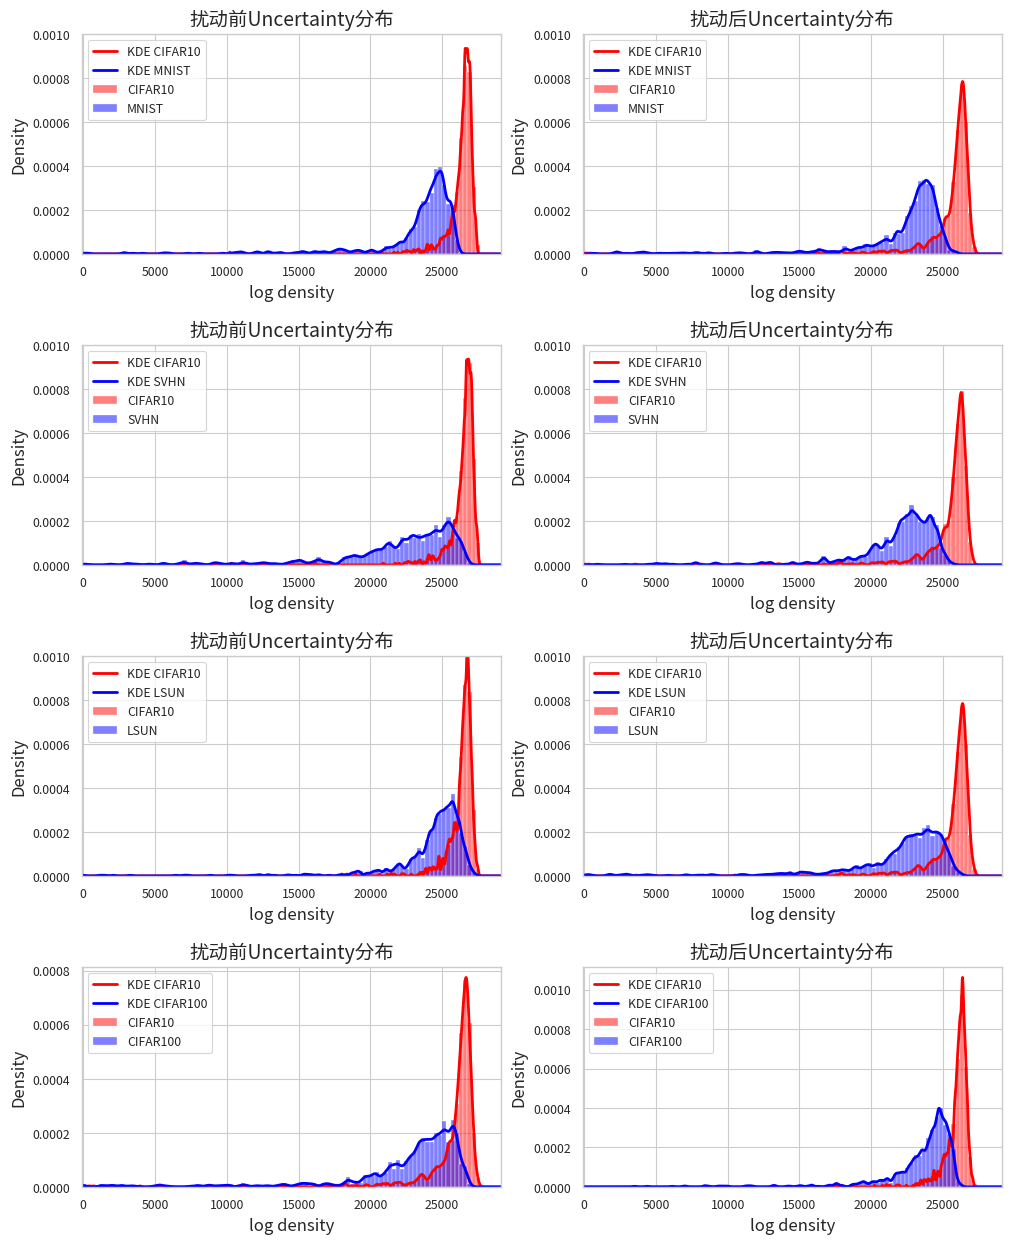
\includegraphics[width=\linewidth]{assets/combined_vertical_image.png}
    \vspace{-1pt} % 可以增加负值来减少下方的空白
    \caption{ResNet50模型 ,训练集 vs OOD数据集,模型不确定性的分布直方图}
    \label{tag:uncertainty 1}
\end{figure}
% \begin{figure}[H]
%     \vspace{-1pt} % 增加负值来减少上方的空白
%     \centering
%     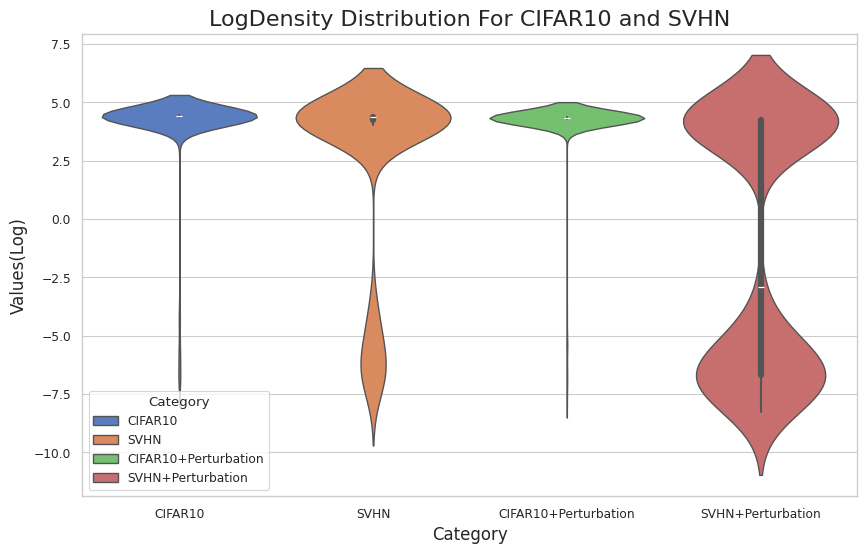
\includegraphics[width=\linewidth]{assets/SVHN_logdensity_violin_purturbation.png}
%     \caption{ResNet50 ,训练集 CIFAR10 vs OOD数据集SVHN,模型不确定性的分布小提琴图}
%     \label{tag:uncertainty 3}
% \end{figure}


% \ref{tag:uncertainty 3}这张图展示了CIFAR10和SVHN两种数据集的对数密度分布(LogDensity),以及添加扰动后的分布变化。原始数据中,CIFAR10的密度值集中在较高区域(0到5),分布紧凑,表明特征分布较为集中;而SVHN的密度范围更广(-7.5到5),分布较为分散,说明其特征噪声更大且类间区分性较低。添加扰动后,CIFAR10的分布范围有所扩展(-10到7.5),但中心变化不大,影响较小;相比之下,SVHN的分布变化更显著,扰动导致其密度分布更对称且范围更大,表明SVHN对扰动更为敏感。这说明CIFAR10特征分布较紧凑,更易分类,而SVHN分布较分散,模型可能需要更强的鲁棒性来应对扰动对特征区分性的影响。


下面从理论上分析,当加入微小输入扰动时,关于最大概率密度的变化,有以下结论:

\textbf{性质2:}
已知 \( z = f_\theta(x) \), \( q(z) = \max_c N(z|\mu_c, \Sigma_c) \),以及 \( U(x) = \log q(z) \)。 \( U(x) \) 对 \( x \) 的梯度 \( \nabla_x U(x) \):\[
\nabla_x U(x) = - \frac{\partial z}{\partial x}^T \Sigma_c^{-1} \left( z - \mu_c \right)
\],对于输入 \( x \) 减去微小的梯度扰动,扰动系数 \( \epsilon \),则:
\[
x' = x - \epsilon \nabla U(x),
\],证明\( x' \) 概率密度下降,且距离均值越远,下降程度越大。

\textbf{证明2:}

多元正态分布的概率密度函数为:
\[
N(z) = \frac{1}{\sqrt{(2\pi)^k |\Sigma|}} \exp\left(-\frac{1}{2}(z - \mu_c)^T \Sigma^{-1} (z - \mu_c)\right),
\]
取对数后可得:
\[
U(x) = \log N(z) = -\frac{k}{2} \log(2\pi) - \frac{1}{2} \log |\Sigma| - \frac{1}{2} (z - \mu_c)^T \Sigma^{-1} (z - \mu_c),
\]
其中 \( z = f(x) \)。

将 \( U(x-\delta) \) 在 \( x \) 附近进行一阶泰勒展开:
\[
U(x-\delta) \approx U(x) - \nabla U(x)^T \delta.
\]
因此:
\[
U(x-\delta) - U(x) \approx - \nabla U(x)^T \delta.
\]

将 \( \delta = \epsilon \nabla U(x) \) 代入,得到:
\[
U(x-\epsilon \nabla U(x)) - U(x) \approx - \epsilon \nabla U(x)^T \nabla U(x).
\]

由于 \( \nabla U(x)^T \nabla U(x) \) 是梯度的二范数平方,故其始终非负:
\[
\|\nabla U(x)\|^2 = \nabla U(x)^T \nabla U(x) \geq 0.
\]
因此:
\[
U(x-\epsilon \nabla U(x)) - U(x) \leq 0.
\]

所以,减去梯度后,概率密度会下降。

根据\textbf{性质3.1},有:
\[
\nabla_x U(x) = - \frac{\partial z}{\partial x}^T \Sigma_c^{-1} \left( z - \mu_c \right).
\]

将其带入 \( -\nabla U(x)^T \nabla U(x) \),展开后可得:
\[
-\nabla U(x)^T \nabla U(x) = -\left[ -\frac{\partial z}{\partial x}^T \Sigma_c^{-1} \left( z - \mu_c \right) \right]^T \left[ -\frac{\partial z}{\partial x}^T \Sigma_c^{-1} \left( z - \mu_c \right) \right].
\]

化简后:
\[
U(x-\epsilon \nabla U(x)) - U(x) \approx
-\nabla U(x)^T \nabla U(x) = -\left( z - \mu_c \right)^T \Sigma_c^{-1} \frac{\partial z}{\partial x} \frac{\partial z}{\partial x}^T \Sigma_c^{-1} \left( z - \mu_c \right),
\]
其中中间的部分是正定的。因此,可以得出结论:距离均值越远,降低程度越大。



下面从理论上分析加入与梯度相关的扰动如何影响模型不确定性,模型不确定性对输入图像的梯度:
\[
\nabla_x U(x) = - \frac{\partial z}{\partial x}^T \Sigma_c^{-1} (z - \mu_c)
\]
这一梯度反映了模型不确定性 \( U(x) \) 如何随着输入 \( x \) 的变化而变化。在扰动过程中,向输入图像施加一个与梯度方向相关的扰动量 \( \epsilon \nabla_x U(x) \),因此新的图像变为 \( x' = x - \epsilon \nabla_x U(x) \),即沿梯度方向反向调整输入。通过这一扰动,输入图像的特征 \( z \) 会发生变化。由于梯度方向是概率密度下降最快的方向,扰动后的图像 \( x' \) 的特征 \( z' \) 会更远离原始均值 \( \mu_c \)。这种调整意味着,扰动后的图像 \( x' \) 将导致概率密度 \( U(x) \) 的值下降。这是因为当特征 \( z' \) 远离均值 \( \mu_c \) 时,\( (z' - \mu_c)^T \Sigma_c^{-1} (z' - \mu_c) \) 的值增大,从而使得 \( U(x') \) 变得更低,表示模型对输入图像的不确定性增大。

具体到实验中的inD样本和OOD样本,扰动作用会影响它们的概率密度。对于inD样本,其特征 \( z \) 初始时与均值 \( \mu_c \) 较为接近,因此概率密度较大,模型的置信度较高。当施加扰动后,尽管扰动使得这些inD样本的特征 \( z' \) 更远离均值,但由于它们本身已经较接近均值,扰动后的变化不会非常剧烈,导致其概率密度的下降幅度相对较小。

与此不同,OOD样本的特征 \( z \) 在原始状态下已经远离均值 \( \mu_c \),因此其初始概率密度较低,表现出较高的不确定性。当对这些样本施加扰动时,它们的特征 \( z' \) 会进一步偏离均值,导致其概率密度迅速下降。由于这些样本初始就处于分布的边缘或尾部,扰动引起的概率密度变化更加显著,因此它们的模型不确定性增加幅度远大于inD样本。

通过这样的扰动作用,可以观察到inD样本和OOD样本的不确定性分布在扰动前后的变化。原本重叠较多的分布,经过扰动后,逐渐拉开了差距。尤其是扰动后,OOD样本的概率密度下降幅度更大,从而使得inD样本和OOD样本的模型不确定性分布差异显著增大。这表明,扰动不仅使得模型对OOD样本的敏感性更高,还提高了模型区分inD样本和OOD样本的能力。

综上所述,梯度扰动的加入使得输入图像的特征 \( z \) 更加偏离均值 \( \mu_c \),从而导致概率密度 \( U(x) \) 下降。对于OOD样本,由于其特征原本就远离均值,扰动的影响更为显著,导致其不确定性增大幅度大于inD样本,从而加大了两者之间的不确定性分布差异。



\section{实验结果与分析}
为了评估本文所提出的基于输入扰动的改进对模型不确定性建模的提升,本节分别在OOD检测任务上,对抗样本检测任务上,误分类样本识别,主动学习等任务上进行了评估。本节的实验内容主要是在CIFAR-10\cite{Krizhevsky2009},CIFAR-100\cite{Krizhevsky2009},SVHN\cite{Netzer2011},MNIST\cite{LeCun1998},LSUN\cite{Yu2015}等数据集和VGG\cite{simonyan2014very},ResNet\cite{he2016deep},VIT\cite{dosovitskiy2020image}等模型进行的,有关实验数据集和模型介绍如下:

\subsubsection{实验数据集介绍}


CIFAR-10(Canadian Institute for Advanced Research 10)是一个广泛用于机器学习和计算机视觉领域的小型图像分类数据集,主要设计用于图像分类任务和模型性能的评估。 CIFAR-10 包含 10 个类别的彩色图像,CIFAR10数据集包含训练集50000 张图片,每类 5000 张,测试集10000 张图片,每类 1000。每张图片的大小为 32 × 32 ,彩色图像。每张图片都有一个对应的标签,用于标注其所属的类别,标签值从 0 到 9,分别对应 10 个类别。

CIFAR-100 数据集是 CIFAR-10 的扩展版,也是一个广泛用于机器学习和计算机视觉任务的小型图像数据集。它具有更复杂的分类任务,适合评估和研究模型在多类别任务中的表现。 CIFAR-100 包含 100 个类别的彩色图像,每个类别的图片属于自然界和日常生活中的常见对象,例如植物、动物、交通工具等。CIFAR-100包含训练集50000 张图片,每类 500 张,测试集10000 张图片,每类 100 张。每张图片的大小为 32 × 32 ,彩色图片。CIFAR-100 提供两种标签:粗粒度标签有20 个粗类别(如哺乳动物、鱼类、家具等),每个粗类别下包含若干个细粒度类别。细粒度标签共100 个细类别,标签值从 0 到 99。

SVHN(Street View House Numbers)数据集是一个常用于机器学习和计算机视觉的公开数据集,主要设计用于识别自然场景中的数字。SVHN数据集由从谷歌街景图片中提取的数字组成,图片内容通常包含街道门牌号码中的数字。目标是识别每张图片中的数字类别(0-9)。SVHN数据集包含训练集73257 张图片,测试集26032 张图片,额外数据集531131 张图片,用于扩展训练数据,图片分辨率为32 × 32 ,都是彩色图片(RGB),标签范围0 到 9。

MNIST(Modified National Institute of Standards and Technology)数据集是机器学习和计算机视觉领域最著名的基准数据集之一,用于手写数字识别任务。 MNIST 数据集包含灰度的手写数字图片,数字范围为 0 至 9(共 10 个类别),训练集有60000 张图片,测试集有10000 张图片,每张图片的分辨率为 28 × 28 ,每张图片都有一个对应的标签,表示其数字类别,标签值为 0 到 9 的整数。


LSUN (Large-scale Scene Understanding) 是一个计算机视觉中的大规模的场景理解任务图像数据集,由中国香港中文大学的视觉计算组(CUImage)创建, 包含了数百万张图像,涵盖了10个不同的类别(如房间、建筑物、场景等),每个类别通常包含大量的标注图像,图像内容大多是场景中的自然环境或人工结构,适合用于训练场景分类、检测等任务。LSUN 分类数据集包含 10 个场景类别,例如餐厅、卧室、鸡、户外教堂等。对于训练数据,每个类别包含大约 120000 到 3000000张图片,验证数据集包括 300 张图像,测试数据集每个类别有 1000 张图像。


\subsubsection{实验模型介绍}
VGG 是由牛津大学 Visual Geometry Group 提出的经典卷积神经网络模型,因其结构简单而广受欢迎。VGG 的核心特点是使用多个 3×3 的小卷积核堆叠代替大卷积核,增加了网络的非线性表达能力,同时保持较少的参数量。VGG16 是其代表性版本,由 16 层有权重的层组成,包括 13 层卷积层和 3 层全连接层。尽管参数量较大(约 138M),VGG 模型凭借高效的特征提取能力,在图像分类和特征迁移任务中表现优异。

ResNet(Residual Network)由微软亚洲研究院提出,通过引入残差结构解决了深度网络中的梯度消失问题,使得网络可以加深到上百层甚至更深。其核心模块是残差块(Residual Block),通过跳跃连接(Skip Connection)将输入直接添加到输出,从而实现“学习残差”的目标。

VIT 是 Google 提出的首个将 Transformer 架构引入计算机视觉的模型,通过处理图像块(Patch)实现全局特征建模。它将图像划分为固定大小的图块,展平后作为序列输入 Transformer 编码器,同时通过位置编码加入空间信息。VIT 擅长在大型数据集上捕获全局依赖关系,与传统卷积网络相比,更加灵活且具有更少的归纳偏置。尽管其对数据量和计算资源的要求较高,但 VIT 在图像分类等任务上展现了超越传统 CNN 的潜力。

本章主要训练了VGG16,ResNet50,VIT三种模型,有关批次,批大小,优化器,初始学习率等超参数设置见下表格\ref{tab:模型训练}。
\begin{table}[htbp]
	\captionsetup{font=small, justification=centering}
	\centering
	\resizebox{\linewidth}{!}{
	\begin{tabular}{c c c c c c c c}
	\hline
	模型结构 & 训练数据集 & 批次 & 批大小 &优化器 & 初始学习率 & 动量 &权重衰减 \\
	\hline
	VGG16 & CIFAR10 & 300 & 512 & SGD & 0.1 & 0.9 & 0.0005 \\
        ResNet50 & CIFAR10 & 300 & 512 & SGD & 0.1 & 0.9 & 0.0005 \\
        VIT & CIFAR10 & 300 & 512 & SGD & 0.01 & 0.9 & 0.0005 \\
	\hline
	\end{tabular}
	}
	\caption{
	模型训练超参数设置
	}
        \label{tab:模型训练}
\end{table}



\subsection{OOD检测任务上评估}
OOD检测任务是指在机器学习和深度学习领域中,模型需要识别输入数据是否属于其训练数据分布范围的任务。OOD样本通常是训练过程中未见过的、不属于目标分布的输入数据,可能来源于其他类别、分布或完全不同的数据集。对于训练集上的分布内样本(In-Distribution, InD)通常具有较低的不确定性,而对于分布外样本(OOD)由于未被训练数据覆盖,模型对其预测的可信度应该较低,应表现为高不确定性。因此,模型不确定值作为OOD检测的指标能否有效地区分ID和OOD样本,可以间接地表征所计算出来的不确定性的值对模型不确定性的建模效果,利用模型不确定性检测OOD样本的规则\ref{eq:uncertainty_rule}所示。本章实验首先是在OOD检测任务上评估基于输入扰动的改进对模型不确定性建模的效果,在CIFAR10数据集的训练集上训练分类模型,选取CIFAR10测试集作为分布内样本(inD),然后选取SVHN,LSUN,MNIST,CIFAR100等数据集作为分布外样本(OOD),使用计算出来的概率密度作为模型不确定性并进行OOD检测,对比扰动前后的不确定性建模的效果。实验结果如表\ref{tag:ood_results_cifar}。

\begin{equation}
x {\rightarrow}
\begin{cases} 
\text{in-domain (inD)} & \text{if } Uncertainty(x) < threshod, \\
\text{out-of-domain (OOD)} & \text{if } Uncertainty(x) > threshold.
\end{cases}
\label{eq:uncertainty_rule}
\end{equation}



\begin{table}[h]
    \captionsetup{font=small, justification=centering}
    \centering
    \renewcommand{\arraystretch}{1.0} % Adjust line spacing
    \resizebox{\linewidth}{!}{
    \begin{tabular}{l l c c c}
    \toprule
    Method & OOD Dataset & VGG16+CIFAR10 & ResNet50+CIFAR10 & VIT+CIFAR10 \\
    &  & (Accuracy=0.9390) & (Accuracy=0.9558) & (Accuracy=0.9732) \\
    \midrule
    \multirow{4}{*}{DDU} 
    & SVHN & \textbf{0.9320} / \textbf{0.9480} & 0.9179 / 0.9415 & 0.9767 / 0.9835 \\
    & LSUN & 0.9160 / \textbf{0.9274} & 0.9239 /0.9390 & 0.9858/0.9886\\
    & CIFAR100 & 0.8932 / 0.9030& 0.8888 / 0.9018 & 0.9476 /\textbf{0.9534} \\
    & MNIST & 0.9195 / 0.9225 & 0.9292 /0.9511& 0.9601 / 0.9684\\
    \midrule
    \multirow{4}{*}{输入扰动的改进方法} 
    & SVHN & 0.9283 / 0.9455 & \textbf{0.9690} / \textbf{0.9731} & \textbf{ 0.9828} / \textbf{0.9867} \\
    & LSUN & \textbf{0.9172} / 0.9266 & \textbf{0.9323}/ \textbf{0.9411} &\textbf{ 0.9929} / \textbf{ 0.9938} \\
    & CIFAR100 & \textbf{0.8938} /\textbf{ 0.9047} &\textbf{ 0.8898} / \textbf{0.9026} & \textbf{0.9491}/ 0.9529 \\
    & MNIST &\textbf{ 0.9482 }/ \textbf{0.9407} & \textbf{0.9757}/ \textbf{0.9813} & \textbf{0.9903 }/ \textbf{0.9919 }\\
    \bottomrule
    \end{tabular}
    }
    \caption{在CIFAR10上训练不同的模型(VGG16,ResNet50,VIT),选取SVHN、LSUN、CIFAR100、MNIST作为OOD样本,对比DDU和梯度范数(GradNorm)对模型不确定性的建模效果,报告指标是AUROC($\uparrow$) / AUPRC($\uparrow$)}
    \label{tag:ood_results_cifar}
\end{table}


从实验结果中可以看出,相比与DDU算法,基于输入扰动的改进在大多数情况下显著提升了OOD 检测性能,在 AUROC 和 AUPRC 两项指标上的表现均优于基础 DDU 方法。实验在不同的模型(VGG16、ResNet50 和 VIT)和 OOD 数据集(如 SVHN、LSUN、CIFAR100 和 MNIST)上,输入扰动均提升了OOD检测的效果。此外,还可以观察到,模型架构对OOD检测结果也有显著影响,VIT 模型在整体表现上优于 VGG16 和 ResNet50,这可能归因于其更复杂的网络具备更强的表征学习能力。综合来看,输入扰动的策略作为对 DDU 方法的改进,不仅提升了模型的不确定性建模能力,还在多种场景下展示了其对鲁棒性的显著作用,具有重要的应用潜力。

实验中还选取MNIST数据集作为训练集,在VGG16/ResNet/VIT等模型上训练,并选取CIFAR10/LSUN/CIFAR100/SVHN作为OOD数据集进行OOD检测,从表\ref{tab:ood_results_mnist}中同样可以看出输入扰动的改进计算出来的不确定性在OOD检测任务上带来的提升,验证了基于输入扰动的改进策略对模型不确定性建模能力的提升。
\begin{table}[h]
    \captionsetup{font=small, justification=centering}
    \centering
    \renewcommand{\arraystretch}{1.0} % Adjust line spacing
    \resizebox{\linewidth}{!}{
    \begin{tabular}{l l c c}
    \toprule
    Method & OOD Dataset & VGG16+MNIST (Accuracy=0.9882) & ResNet50+MNIST (Accuracy=0.9870) \\
    \midrule
    \multirow{4}{*}{DDU} 
    & CIFAR10 & 0.9949 / 0.9964 & 0.9949 / 0.9964 \\
    & LSUN & 0.9946 / 0.9962 & 0.9946 / 0.9962 \\
    & CIFAR100 & 0.9945 / 0.9961 & 0.9945 / 0.9961 \\
    & SVHN & 0.9941 / 0.9960 & 0.9941 / 0.9960 \\
    \midrule
    \multirow{4}{*}{输入扰动的改进方法} 
    & CIFAR10 & \textbf{0.9965} / \textbf{0.9974} & \textbf{0.9965} / \textbf{0.9974} \\
    & SVHN & \textbf{0.9963} / \textbf{0.9972} & \textbf{0.9963} / \textbf{0.9972} \\
    & CIFAR10 & \textbf{0.9961} / \textbf{0.9970} & \textbf{0.9961} / \textbf{0.9970} \\
    & SVHN & \textbf{0.9964} / \textbf{0.9973} & \textbf{0.9964} / \textbf{0.9973} \\
    \bottomrule
    \end{tabular}
    }
    \caption{在CIFAR10上训练不同的模型(VGG16,ResNet50,VIT),选取SVHN、LSUN、CIFAR100、MNIST作为OOD样本,对比DDU和梯度范数(GradNorm)对模型不确定性的建模效果,报告指标是AUROC($\uparrow$) / AUPRC($\uparrow$)}
    \label{tab:ood_results_mnist}
\end{table}



\subsubsection{各种方法的对比}
在实验中,使用ResNet50模型在CIFAR10数据集上进行训练,选取不同数据集(CIFAR100、LSUN、MNIST和SVHN)作为OOD样本,并通过对比几种常用的不确定性建模的方法在OOD检测任务上的表现,来观察基于输入扰动的改进所带来的提升。实验中选择了四种不确定性建模方法:MSP、集成方法(Ensemble)、DDU和 本文提出的基于输入扰动的改进方法,并以AUROC和AUPRC作为评价OOD检测的指标,越高说明对不确定性建模效果越好,实验中MSP方法使用最大Softmax概率作为不确定性的度量,模型集成类方法在不同的数据集增强策略和参数初始化条件下训练了5个模型,模型集成方法使用多次预测的概率的熵作为不确定性的度量,DDU算法和基于输入扰动的改进方法都是在训练集上建模GMM分布并使用测试样本的概率密度作为不确定性的度量。所有的实验结果见表\ref{tab:不同方法的对比}。


从实验结果可以看出,DDU算法作为单一确定性神经网络建模不确定性的算法,虽然具有存储空间小和计算高效等优点,但是对不确定性建模的效果相比模型集成类的方法还有差距,整体上来看模型集成类的算法在OOD检测任务上表现是优于DDU算法的。同时可以观察到,加入输入扰动后,在OOD检测任务上在多个数据集上取得了最佳的AUROC/AUPRC值,甚至在MNIST和SVHN数据集上超过了过去最优的建模不确定性的算法模型集成类的方法。综合实验结果,可以得出结论:输入扰动的改进方法在OOD检测任务中显著优于传统的MSP和DDU算法,提升了对不确定性的建模能力。
% \begin{table}[htbp]
% 	\captionsetup{font=small, justification=centering}
% 	\centering
% 	\resizebox{\linewidth}{!}{
% 	\begin{tabular}{c c c c c}
% 	\hline
% 	OOD Dataset & MSP (AUROC/AUPRC) & Ensemble (AUROC/AUPRC) & DDU (AUROC/AUPRC) & DDU+ip (AUROC/AUPRC) \\
% 	\hline
% 	CIFAR100 & 0.8925/0.8995 &\textbf{0.9184}/\textbf{0.9167} & 0.8888 / 0.9018 & 0.8898 / 0.9026\\
% 	LSUN & 0.9120/0.9238 & \textbf{0.9401}/0.9265 & 0.9239 /0.9390 & 0.9323/ \textbf{0.9411} \\
% 	MNIST & 0.9471/0.9573 & 0.9735/0.9706 &0.9292 /0.9511 &  \textbf{0.9757}/ \textbf{0.9813} \\
% 	SVHN & 0.9392/0.9405 & 0.9667/0.9599 & 0.9179 / 0.9415 & \textbf{0.9690} / \textbf{0.9731}  \\
% 	\hline
% 	\end{tabular}
% 	}
% 	\caption{
% 	在CIFAR10上训练ResNet50模型, 在OOD检测任务上对比各种方法的结果,报告指标是AUROC($\uparrow$) / AUPRC($\uparrow$)
% 	}
%         \label{tab:不同方法的对比}
% \end{table}

\begin{table}[htbp]
	\captionsetup{font=small, justification=centering}
	\centering
	\resizebox{\linewidth}{!}{
	\begin{tabular}{c c c c c}
	\hline
	inD/OOD Dataset & Method & 不确定性计算方式 & AUROC & AUPRC \\
	\hline
	\multirow{4}{*}{CIFAR10/CIFAR100} & MSP & 最大预测概率 & 0.8925 & 0.8995 \\
	 & Ensemble & 熵 & \textbf{0.9184} & \textbf{0.9167} \\
	 & DDU & 概率密度 & 0.8888 & 0.9018 \\
	 & \textbf{输入扰动的改进} & 概率密度 & 0.8898 & 0.9026 \\
	\hline
	\multirow{4}{*}{CIFAR10/LSUN} & MSP & 最大预测概率 & 0.9120 & 0.9238 \\
	 & Ensemble & 熵 & \textbf{0.9401} & 0.9265 \\
	 & DDU & 概率密度 & 0.9239 & 0.9390 \\
	 & \textbf{输入扰动的改进} & 概率密度 & 0.9323 & \textbf{0.9411} \\
	\hline
	\multirow{4}{*}{CIFAR10/MNIST} & MSP & 最大预测概率 & 0.9471 & 0.9573 \\
	 & Ensemble & 熵 & 0.9735 & 0.9706 \\
	 & DDU & 概率密度 & 0.9292 & 0.9511 \\
	 & \textbf{输入扰动的改进} & 概率密度 & \textbf{0.9757} & \textbf{0.9813} \\
	\hline
	\multirow{4}{*}{CIFAR10/SVHN} & MSP & 最大预测概率 & 0.9392 & 0.9405 \\
	 & Ensemble & 熵 & 0.9667 & 0.9599 \\
	 & DDU & 概率密度 & 0.9179 & 0.9415 \\
	 & \textbf{输入扰动的改进} & 概率密度 & \textbf{0.9690} & \textbf{0.9731} \\
	\hline
	\end{tabular}
	}
	\caption{
	在CIFAR10上训练ResNet50模型, 在OOD检测任务上对比各种方法的结果,报告指标是AUROC($\uparrow$) / AUPRC($\uparrow$)
	}
        \label{tab:不同方法的对比}
\end{table}


    
\subsection{误分类样本检测任务上评估}
神经网络通常会在训练数据上表现出良好的性能,但在测试数据或分布外样本上可能会产生错误预测,误分类样本检测任务用于评估神经网络在预测结果上的不确定性,是通过模型能否依据不确定性值识别出自身预测可能不准确的样本。如果模型能够有效地评估自身的不确定性,就可以标记出潜在的误分类样本,从而提醒用户或触发更进一步的处理(例如人工复核)。在误分类检测任务上评估神经网络不确定性建模效果,对测试集样本进行预测,根据预测结果是否正确分为正确预测和错误预测两个类别,然后通过计算出的模型不确定性作为二分类的指标,区分测试样本为正确分类和错误分类两个类别,如果所计算的模型不确定性在这个二分类任务上表现的越好,说明对模型不确定性建模效果越好。

本节在VGG/ResNet50/VIT等训练的不同模型进行误分类检测实验。如图\ref{tab:misclassified},实验结果表明,加入输入扰动(InputPerturbation)的改进方法在所有模型上均显著提升了 AUROC 和 AUPRC 指标,特别是在 ResNet50 和 VIT 模型中效果尤为突出。这表明输入扰动能够有效增强模型对误分类样本和分布外样本(OOD)的检测能力,提高模型的不确定性估计性能。

同时本实验评估了加入输入扰动前后模型的校准性能,该性能由ECE指标表示,从表\ref{tab:misclassified}中可以看出,加入输入扰动(InputPerturbation)的改进方法在所有模型上在ECE指标上均降低了,ECE指标越低表明模型的预测概率与实际准确率之间的匹配程度较好,即模型是校准良好的,由此得出结论:基于输入扰动的改进方法能够提高模型的校准性能。
\begin{table}[h]
    \captionsetup{font=small, justification=centering}
    \centering
    \renewcommand{\arraystretch}{1.0} % Adjust line spacing
    \resizebox{\linewidth}{!}{
    \begin{tabular}{l l c c c}
    \toprule
    Method & Model & AUROC($\uparrow$) & AUPRC($\uparrow$) & ECE($\downarrow$) \\
    \midrule
    \multirow{5}{*}{\vspace{4em} DDU} 
    & VGG16 & 0.9274  & 0.9945 & 0.0404\\
    & ResNet50 &  0.9344 & 0.9963 & 0.0286 \\
    & VIT & 0.9481 & 0.9984 &0.0167 \\
    \midrule
    \multirow{5}{*}{\vspace{4em} 输入扰动的改进方法} 
    & VGG15 & \textbf{0.9354} & \textbf{0.9955} & \textbf{0.0385} \\
    & ResNet50 & \textbf{0.9460}  & \textbf{0.9968} &\textbf{0.0262}\\
    & VIT & \textbf{0.9578}  & \textbf{0.9989} &\textbf{0.0138}\\
    \bottomrule
    \end{tabular}
    }
    \caption{误分类样本识别任务,实验结果在不同的模型(VGG16、ResNet50、VIT)上做实验对比DDU和基于输入扰动的改进方法对模型不确定性的建模效果,报告指标是AUROC($\uparrow$) / AUPRC($\uparrow$)/ECE($\downarrow$)}
    \label{tab:misclassified}
\end{table}



\subsection{对抗样本检测任务上评估}
对抗攻击(Adversarial Attack)是机器学习和深度学习领域中的一种模型安全性问题,它指的是通过对输入数据进行不可察觉的扰动,从而使得模型产生错误的预测。对抗攻击揭示了深度学习模型的脆弱性,尤其在计算机视觉、自然语言处理和语音识别等领域。对神经网络进行攻击的算法,包括黑盒攻击和白盒攻击,黑盒攻击不知道模型的内部信息,白盒攻击知道模型的内部信息,在白盒攻击算法中有一类很重要的基于梯度的攻击算法,其中有FGSM、PGD 和 BIM 是三种经典的攻击方式。FGSM (Fast Gradient Sign Method) 是一种单步攻击方法,利用模型的梯度信息生成对抗样本。其攻击方式为:
    \[
    x_{\text{adv}} = x + \epsilon \cdot \text{sign}(\nabla_x J(x, y)),
    \]
    其中 $x$ 是原始输入,$y$ 是正确标签,$\epsilon$ 是扰动强度,$J(x, y)$ 是模型的损失函数。FGSM 的优点是计算效率高,但攻击性较弱。   BIM (Basic Iterative Method) 是 FGSM 的扩展版本,也是一种迭代攻击方法。BIM 在每次迭代中根据梯度更新对抗样本,公式类似 PGD,但通常不包含投影操作。相比 FGSM,BIM 可以生成更强的对抗样本。
   PGD (Projected Gradient Descent)是一种迭代攻击方法,基于 FGSM,通过多次迭代优化生成更强的对抗样本。PGD 在每一步更新后将对抗样本投影到一个 $\epsilon$-球中,以限制扰动幅度。其公式为:
    \[
    x_{\text{adv}}^{t+1} = \Pi_{\epsilon}(x_{\text{adv}}^t + \alpha \cdot \text{sign}(\nabla_x J(x_{\text{adv}}^t, y))),
    \]
    其中 $\Pi_{\epsilon}$ 表示投影操作,$\alpha$ 是每步更新强度。

torchattacks\cite{kim2020torchattacks} 是一个基于 PyTorch 的对抗攻击库,旨在为研究人员和开发者提供简单、易用且高效的对抗攻击方法。它由 Hoki Kim 开发,于 2020 年首次发布,并持续更新。该库支持多种常见的对抗攻击算法,适用于深度学习模型的鲁棒性评估和对抗训练研究。在实验中,本文使用torchattacks实现了对数据的FGSM/BIM/PGD等攻击。

实验中,本文在CIFAR10数据集的测试集上进行攻击,然后使用概率密度作为模型不确定性的度量,并作为对抗样本检测任务的检测指标,对抗样本检测任务本质上也是一个二分类任务,通过检测指标判定测试样本属于原始样本还是被攻击的样本,所以同OOD样本检测一样,最终结果也可以使用AUROC/AUPRC两个指标衡量,AUROC/AUPRC越高,说明在对抗样本检测任务上的性能越好,进而体现了在模型不确定性建模上的效果。实验结果如表\ref{tag:adv detection}



\begin{table}[h]
        \captionsetup{font=small, justification=centering}
	\centering
        \renewcommand{\arraystretch}{1.0} % Adjust line spacing
        \resizebox{\linewidth}{!}{
	\begin{tabular}{llrr}
		\hline
		Method      & Attack Method  & AUROC($\uparrow$)  & AUPRC($\uparrow$)   \\
		\hline
		\multirow{4}{*}{DDU} 
		& FGSM & 0.8428 & 0.8394 \\
		& BIM  & 0.8070 & 0.8816 \\
		& PGD  & 0.7420 & 0.8021 \\
		\hline
		\multirow{4}{*}{input Perturbation} 
		& FGSM & \textbf{0.8882} & \textbf{0.9737} \\
		& BIM   & \textbf{0.8559} & \textbf{0.9686} \\
		& PGD   & \textbf{0.8433} & \textbf{0.9700} \\
		\hline
	\end{tabular}
    }
	\caption{VGG16 + CIFAR10, 对抗样本的检测任务}
        \label{tag:adv detection}
\end{table}



该表格评估了不同的不确定性建模方法在对抗样本检测任务中的效果,表格展示了两种方法(DDU 和 DDU+Input Perturbation)在三种不同的对抗攻击方式(FGSM、BIM 和 PGD)下的 对抗样本检测的结果,并以AUROC/AUPRC作为报告指标。在本实验中攻击的模型为 VGG16,该模型数据集CIFAR10上训练并达到较高的模型准确率。从表格中的结果可以看出,基于输入扰动的改进方法相比于仅使用 DDU 的方法在所有攻击方式下都显著提高了 AUROC/AUPRC 指标,特别是在对抗攻击强度较大的情况下(如PGD攻击),基于输入扰动的改进取的的提升尤为突出。这表明,加入输入扰动的策略在对抗样本检测中发挥了重要作用,尤其在PGD攻击这种较为复杂的攻击方式下,能够显著提高检测效果。在对抗样本检测任务中,输入扰动的加入显著提升了模型的检测能力,在面对不同类型的对抗攻击时,表现稳健且有效。基于输入扰动的模型在对抗样本检测任务上所带来的提升,进一步证实了基于输入扰动的改进在对模型不确定建模上具有更好的性能。
\subsection{主动学习任务上评估}
主动学习是一种机器学习策略,特别适用于标注成本较高的场景。通过主动选择最有价值的数据点来进行标注,可以在使用较少标注数据的情况下显著提升模型性能。主动学习的核心思想是:模型并不需要学习所有数据,只需关注对当前模型改进最有帮助的数据点。初始训练时使用一个小规模的初始标注数据集训练初始模型。之后从未标注的数据集中挑选出最有价值的数据点。这些数据点的选择通常基于模型的不确定性或代表性。将选中的数据点送给专家或标注系统进行标注。将新标注的数据加入训练集,重新训练模型。重复上述过程,直到达到目标性能或资源限制。

在主动学习中,模型会根据当前的模型状态来选择数据样本,这些样本对于模型性能提升最为关键。通过这种方法,模型能够在标注成本高昂或数据标注困难的情况下,尽可能减少标注样本的数量,同时提高准确性。通过主动学习任务评估不确定性建模的质量,是通过选择模型预测最不确定的样本并添加到训练集中重新训练,经过若干次迭代后达到的准确率越高,说明依据不确定性选取样本进行标注并添加到训练集所带来的准确率提升越大,间接表明对不确定性的建模效果。

\begin{figure}[h]
    \captionsetup{font=small, justification=centering}
    \centering
    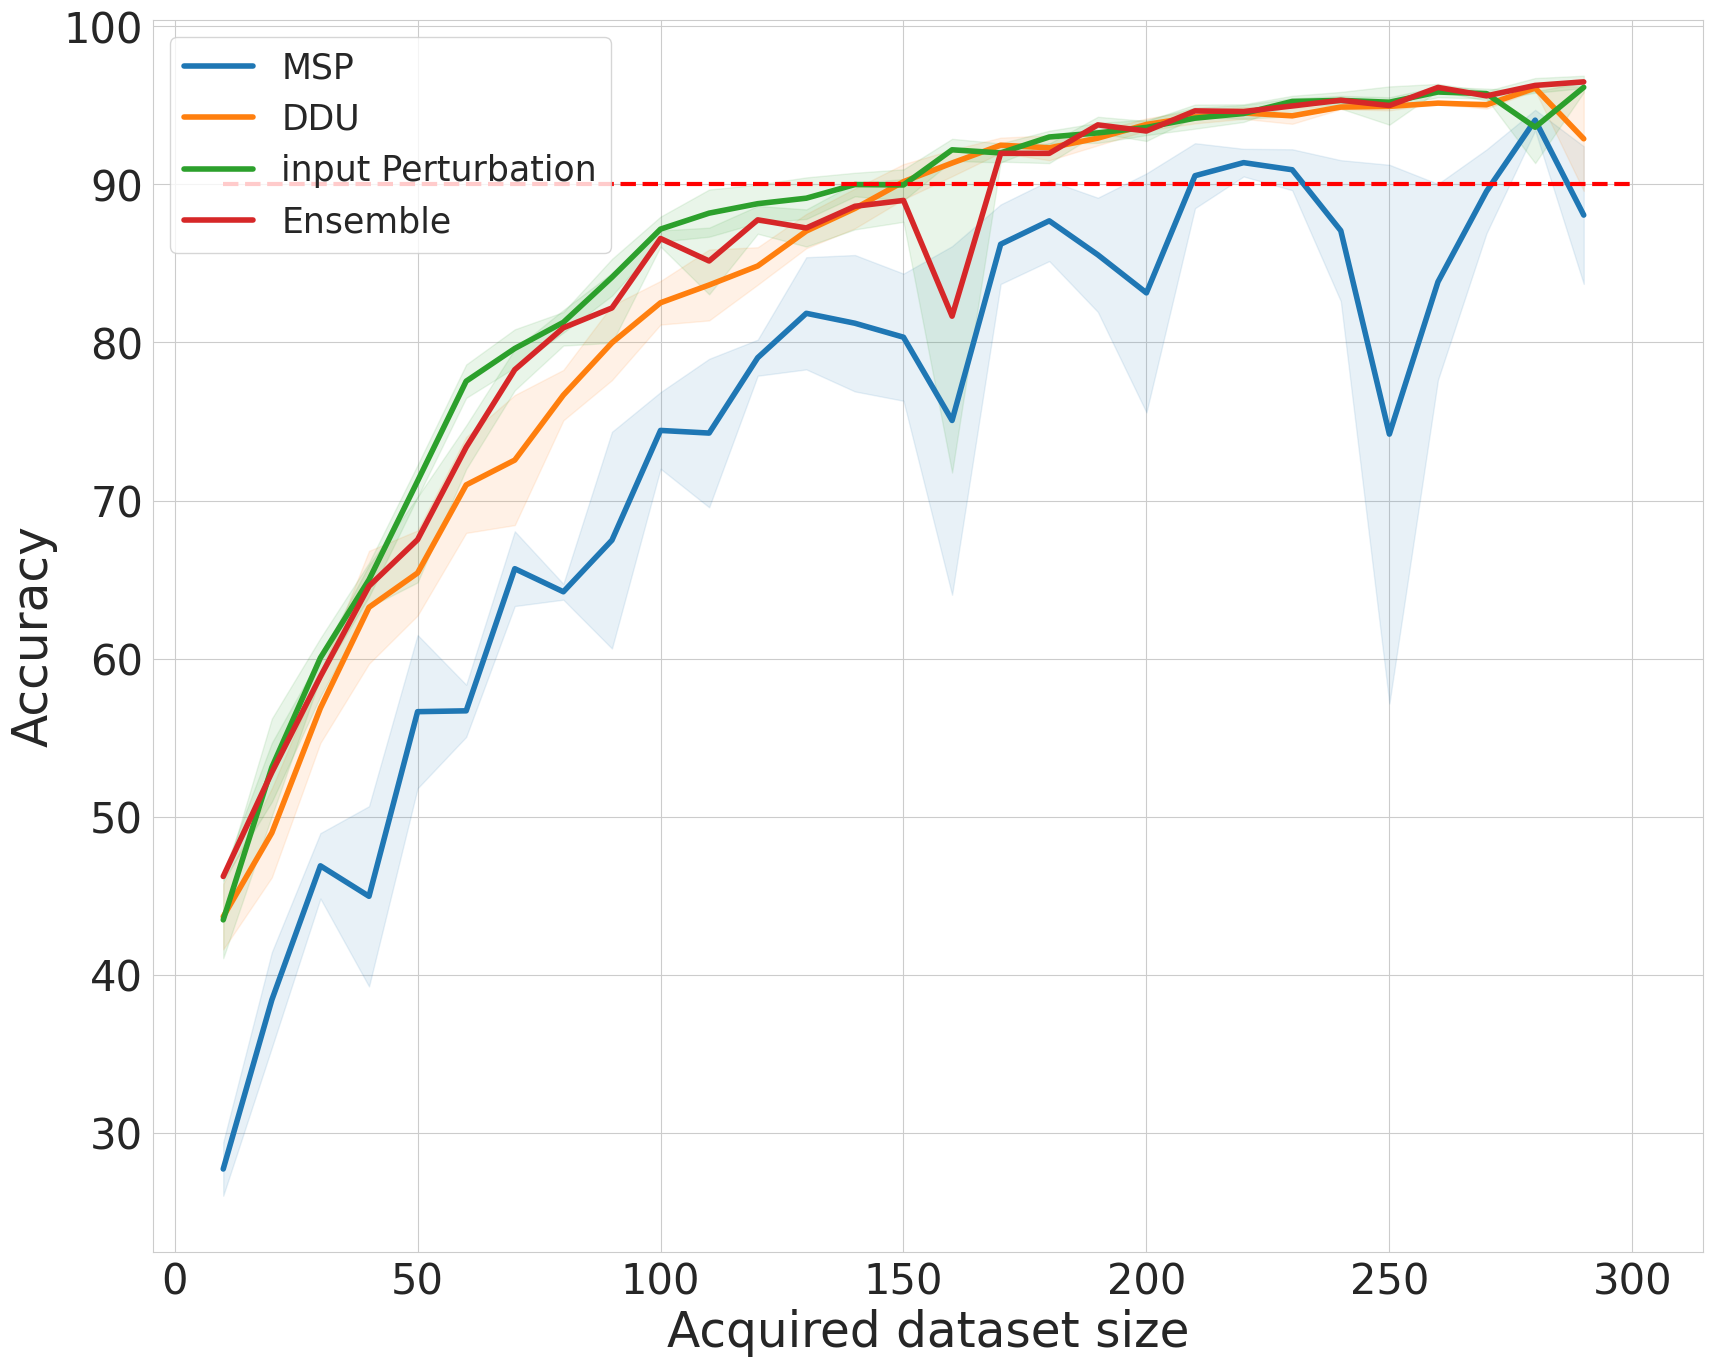
\includegraphics[width=0.75\linewidth]{assets/mnist_test_accuracy_active_learning.png}
    \caption{MNIST数据集,VGG16模型,主动学习任务上对比MSP,DDU,模型集成,基于输入扰动的改进等方法}
    \label{fig:active learning}
\end{figure}
在本实验中,在 MNIST 数据集上训练了 VGG16 模型,并将 MNIST 训练集分为两部分:一部分数据加入已标注的集合,另一部分作为候选池。初始时,已标注集合仅包含 20 个标注样本,模型首先在这些已标注样本上进行训练。随后,每次训练完成后,从候选池中选择模型不确定性最大的 10 个样本,并将其添加到已标注集合中,直到已标注集合的样本数量达到 300 个。在实验过程中,记录了每次训练完成后,模型在测试集上的准确率。实验结果如图 \ref{fig:active learning} 所示。

图 \ref{fig:active learning} 对比了四种模型不确定性建模方法:MSP,模型集成,DDU和本章提出的基于输入扰动的改进方法。图表展示了不同方法在主动学习任务中,随着数据集大小增加,MNIST 测试集准确率的变化趋势。横轴表示采集的数据集大小,纵轴表示 MNIST 测试集的准确率。实验结果表明,在相同的数据集大小下,基于输入扰动的改进方法在测试集上达到了最优的准确率,其次是模型集成方法,接着是 DDU 算法,最后是 MSP 方法。此结果表明,通过模型不确定性选择样本并将其加入已标注集合中,基于输入扰动的改进方法所选样本的价值最大,从而在建模模型不确定性的效果上,基于输入扰动的改进方法优于模型集成方法、DDU 算法和 MSP 方法。

\subsection{消融实验}
消融实验(Ablation Study)是机器学习和深度学习研究中常用的一种分析方法,用于评估模型中各个组件或设计选择的贡献及其对整体性能的影响。通过逐步移除(或替换)某些模块、特征或机制,观察模型性能的变化,从而帮助研究者理解每个部分的重要性和作用。在本节的实验中,本文对比了使用GMM和KDE\cite{davis2011remarks}(Kernel Density Estimation,核密度估计)两种不同的概率密度估计方式,并且对比了高为特征维度对模型不确定性建模的影响。

核密度估计是一种非参数化的概率密度估计方法,用于估计所给数据的概率密度函数(PDF)。给定一组独立同分布的样本点 $\{x_1, x_2, \ldots, x_n\}$,核密度估计的表达式如下:

\[
\hat{f}(x) = \frac{1}{n h} \sum_{i=1}^n K\left(\frac{x - x_i}{h}\right)
\]

其中:$x$ 是我们希望估计概率密度的点,$n$ 是样本数量,$h > 0$ 是带宽(平滑参数),控制核函数的扩展范围。$K(\cdot)$ 是核函数,通常满足以下性质: (1)非负性:$K(u) \geq 0, \forall u \in \mathbb{R}$,(2)积分为1:$\int_{-\infty}^\infty K(u) \, du = 1$,(3)对称性:$K(u) = K(-u)$。常用的核函数包括:高斯核(Gaussian Kernel),均匀核(Uniform Kernel),三角核(Triangle Kernel)。带宽 $h$ 是核密度估计中最重要的参数之一,如果 $h$ 过大,估计会过于平滑,丢失数据的细节。如果 $h$ 过小,估计会出现过拟合现象,导致噪声被放大。在本节的实验中,KDE选用的核函数是高斯核函数,其形式是\[K(u) = \frac{1}{\sqrt{2\pi}} e^{-\frac{u^2}{2}}\],带宽参数h通过交叉验证的方式选取最优值。

\begin{table}[h]
   \captionsetup{font=small, justification=centering}
    \centering
    \resizebox{\linewidth}{!}{
    \begin{tabular}{P{3cm} P{3cm} P{3cm} P{3cm} P{3cm}}
    \hline
    OOD Dataset & \makecell{AUROC/AUPRC\\(D=2048)} & \makecell{AUROC/AUPRC\\(D=1024)} & \makecell{AUROC/AUPRC\\(D=512)} & \makecell{AUROC/AUPRC\\(D=256)} \\
    \hline
    SVHN+GMM & \textbf{0.9179} / \textbf{0.9415} & \textbf{0.9322}/\textbf{0.9508} & 0.9310/0.9503 & 0.9320/0.9516 \\
    LSUN+GMM & \textbf{0.9239 }/ \textbf{0.9390} & \textbf{0.9353}/\textbf{0.9425} & \textbf{0.9363}/\textbf{0.9401} & \textbf{0.9332}/\textbf{0.9305} \\
    CIFAR100+GMM &\textbf{ 0.8888 }/ \textbf{0.9018}  & \textbf{0.9056}/\textbf{0.9131} & \textbf{0.9003}/\textbf{0.9066} & 0.8994/0.9021 \\
    MNIST+GMM &\textbf{ 0.9292 }/\textbf{0.9511}& \textbf{0.9439}/\textbf{0.9602} & 0.9342/0.9548 & 0.9308/0.9516 \\
    
    \hline
    SVHN+KDE & 0.8972/0.9168 & 0.9277/0.9496& \textbf{0.9320}/\textbf{0.9521} & \textbf{0.9422}/\textbf{0.9587} \\
    LSUN+KDE & 0.8957/0.9013 & 0.9199/0.9303 & 0.9218/0.9291 & 0.9278/0.9336 \\
    CIFAR100+KDE & 0.8380/0.8526 & 0.8837/0.9022 & 0.8905/0.9055 & \textbf{0.9013}/\textbf{0.9086} \\
    MNIST+KDE & 0.9151/0.9370 & 0.9370/0.9551& \textbf{0.9404}/\textbf{0.9570} & \textbf{0.9592}/\textbf{0.9596} \\
    \hline
    \end{tabular}
    }
    \caption{
    ResNet50+CIFAR10训练, 不同的概率密度建模方式GMM vs KDE, AUROC ($\uparrow$) and AUPRC ($\uparrow$), 选取的不同的特征维度:2048, 1024, 512和256.
    }
    \label{tag:gmmkde}
\end{table}





在本节实验中对比了所提取的高维特征在不同维度下,基于ResNet50模型在CIFAR10上训练后,使用GMM和KDE两种概率密度估计方法构建分布,在OOD检测任务中的性能。实验选取OOD检测任务间接评估模型不确定性的建模能力,选取了四个不同的OOD数据集(SVHN, LSUN, CIFAR100, MNIST),并以AUROC/AUPRC为报告指标,AUROC/AUPRC越高说明在OOD检测任务上的性能越好。实验结果见表格\ref{tag:gmmkde},并依据表格中的结果绘制折线图如图\ref{fig:gmmkde2}。
\begin{figure}[h]
    \captionsetup{font=small, justification=centering}
    \centering
    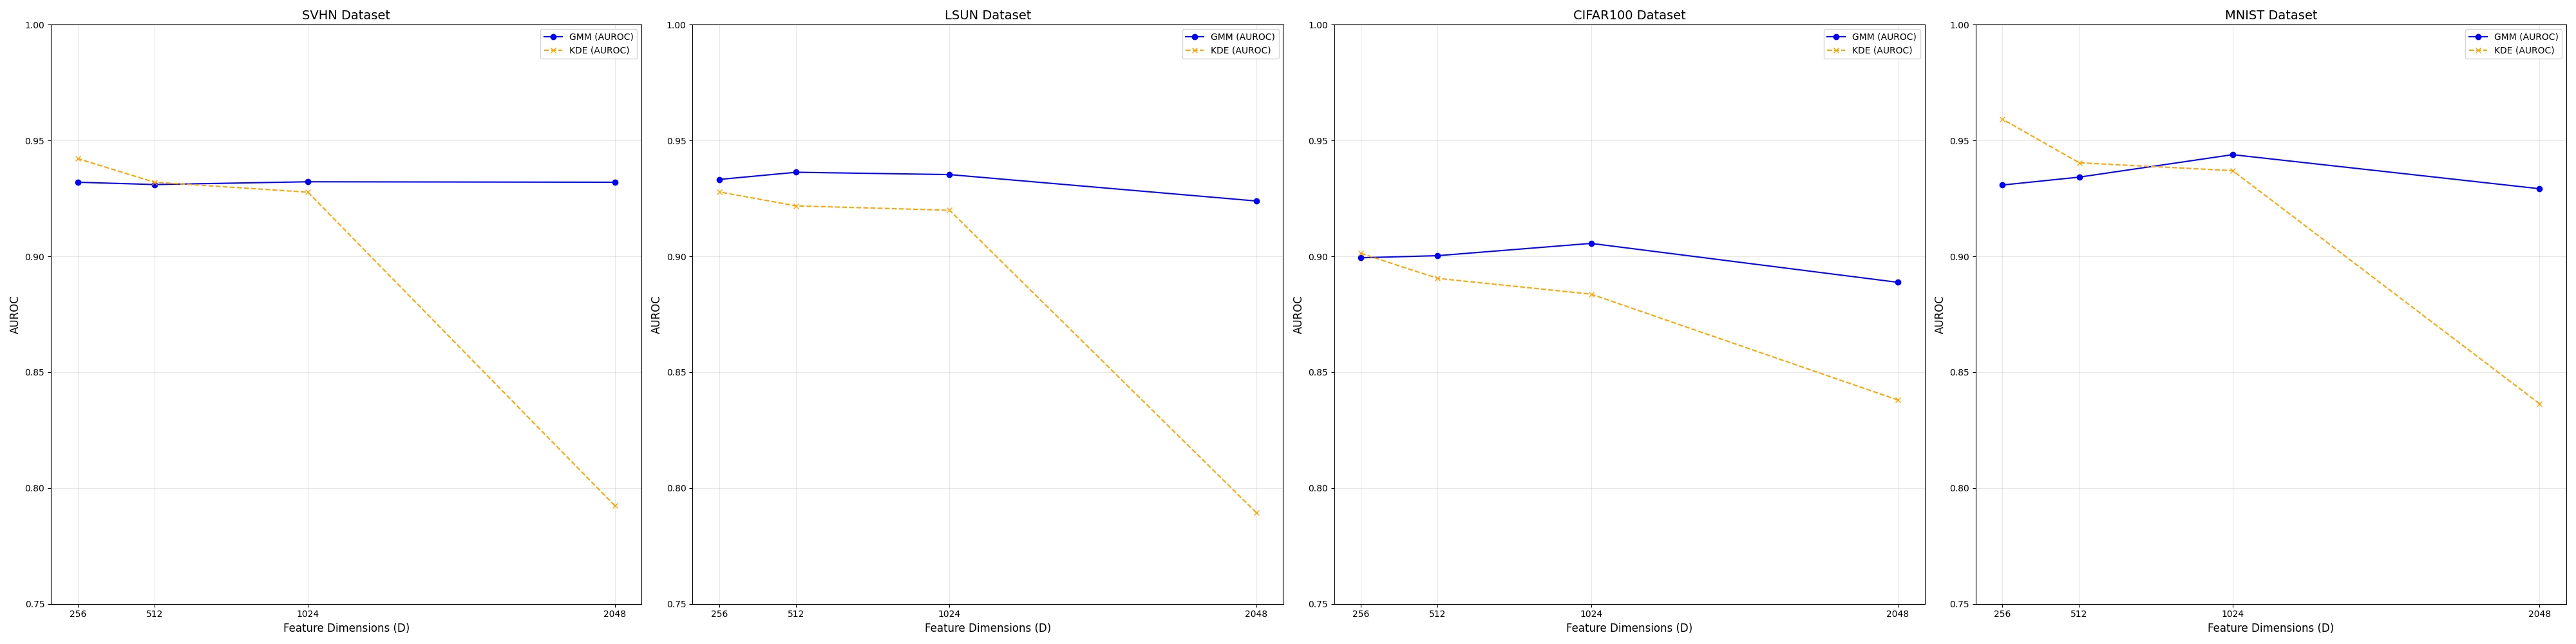
\includegraphics[width=0.9\linewidth]{assets/gmm_kde_dimension.png}
    \caption{ResNet50+CIFAR10训练, 不同的概率密度建模方式GMM vs KDE, AUROC ($\uparrow$) and AUPRC ($\uparrow$), 选取的不同的特征维度:2048, 1024, 512和256.}
    \label{fig:gmmkde2}
\end{figure}

从表格中可以看到,在不同维度(2048, 1024, 512, 256)下,使用GMM和KDE方法的表现有所不同。总体来看,在特征维度比较高时(D=2048),使用GMM构建概率分布的结果完全优于使用KDE构建概率分布,此时使用GMM构建概率分布在不同的OOD检测任务中都表现出更高的AUROC和AUPRC值,在较低维度(D=256)下,使用KDE构建概率分布的结果在大部分OOD检测任务上优于使用GMM构建概率分布,此时使用KDE构建概率分布在不同的OOD检测任务中表现出更高的AUROC和AUPRC值。在不同的OOD检测任务中,随着维度的减少,使用KDE构建概率分布所取得结果在逐渐变好,尤其是在256维时,KDE在大部分数据集上都取得了最好的结果。因此,选择适当的特征维度和不同的分布构建方法(GMM或KDE)对模型不确定性的建模至关重要。

由上述实验可以得出结论,特征维度较低时,使用KDE构建概率分布结果更好,但是特征维度高的时候,使用GMM构建概率分布效果更好。分析其中的原因,可能是因为在低维空间中,KDE得益于其非参数特性,不假设数据分布形状,能够充分利用每个点,有效地捕捉数据的局部结构和分布,但是随着数据维度的增加,样本数据密度变得更加稀疏,发生维度灾难(Curse of Dimensionality)\cite{murphy2012machine},经验分布无法捕捉到真实分布的结构, KDE的表现会下降。在高维数据中GMM具有数据符合高斯分布的先验假设,每个高斯分布可以通过调整均值、方差和权重来捕捉数据的分布,在高维空间中通过依赖协方差矩阵建模维度间的关系,能够适当捕捉相关性,不会受到高维稀疏性的强烈影响。而且,GMM通过参数(均值、协方差矩阵和权重)来定义分布,相比于KDE,避免了KDE的计算瓶颈。 


\section{本章小结}




传统的模型集成方法建模不确定性虽然效果较好,但由于计算和存储开销大,单一模型的不确定性建模方法逐渐受到关注。为高效建模不确定性,本章基于高维特征概率密度建模的不确定性度量展开研究。DDU算法作为其中的一个代表,通过高斯混合模型在高维特征空间上构建概率密度分布并计算概率密度来度量不确定性,然而,DDU算法在某些复杂网络架构和数据集上表现相对集成方法仍有提升空间。

针对DDU算法存在的问题,本章通过分析神经网络的梯度空间,探讨了分布内样本和分布外样本在梯度响应上的差异性。实验结果表明,分布外样本在梯度响应图上的梯度较大,这一现象表明梯度信息与模型不确定性密切相关。基于这一观察,本章提出了基于输入扰动的改进方法,通过对输入样本施加与梯度响应相关的微小扰动,进一步放大了分布内样本和分布外样本在多维概率分布上的差异。输入扰动的引入能够使得域内样本和域外样本在经过高斯混合模型建模的高维特征空间中表现出更为显著的分布差异,从而在不确定性度量中更好地区分异常样本。这一方法可以有效地改善DDU算法在不同数据集上的不确定性建模能力,尤其是在OOD检测、误分类样本识别和对抗样本检测等任务中表现出色。



在理论分析方面,本章通过推导和分析概率密度关于输入的梯度性质,揭示了输入扰动对模型不确定性度量的影响。输入扰动沿着梯度方向进行调整,会使得分布外样本的特征向量远离类别均值,从而使得其在多维概率分布上的概率密度值下降,进一步增强了模型对不确定性的敏感性。通过这种方式,输入扰动有效提高了不确定性建模的能力,尤其是在处理OOD样本时,能够明显增加OOD样本与InD样本在不确定性分布上的差异。

最后,通过消融实验,本章还对比了KDE和高斯混合模型两种不同的概率密度建模方式,在模型不确定性上的表现,实验表明高斯混合模型在高维特征上是一种更稳定有效的概率密度建模方式。

本章的研究提出了基于输入扰动的神经网络模型不确定性建模方法,并且通过实验验证了其有效性。这一方法为提高深度学习模型在高风险领域的应用提供了新的思路和技术支持,尤其是在需要进行不确定性度量和风险控制的场景中具有重要的实际应用价值。

